% !TEX root = thesis.tex



\section{Results}
In this section, we show experimental results for two prediction tasks, predicting speaking status and social formations, from different input sources. The core direction in performing this experiments is to explore the correlations of diverse behavioral channels measured in genuine social communications by leverage the broad spectrum of social signal measurements of the Haggling dataset.

\subsection{Pre-processing Haggling Data}
Given the measurement data of the Haggling games described in Chapter~\ref{chapter:dataset}, we first manually annotate the start and end time of the game, where the start time is decided when the social formation is built and the end time is defined when the social formation is broken. We crop out the motion dataset based on this start and end time, so that we ignore the time while subjects enter and exit the capture space. For each haggling game scene, we also annotate the roles in the game, buyer, left-seller, and right-seller, where the left and right are determined in the buyer's viewpoint. In our experiment, we specify that the left seller is our target person and predict the social behavior of these subjects. As described in our method section, we re-target the motion data to a standardized skeleton size to remove size variation from the body skeletons. We also synthesize footstep signals and decouple the body motion from global translation and orientation using the method of \cite{holden2016deep}. For face motion, we fit the face part of our Adam model (described in Chapter~\ref{chapter:totalcapture}) on the 3D keypoints of individual's face, and use the first five facial expression parameters, as described in our method section. Finally, we divide the dataset into 140 training sets and 40 test sets. However, since there exist sequences where the reconstruction errors are severe for some frames, we select only 79 training sets and 28 testing sets which are manually verified to be error free. We additionally divide all training set into slices with 120 frames to train our models. We standardize all input data so that they have zero mean and unit variance.


%\begin{figure}[t]
%	\centering       
%	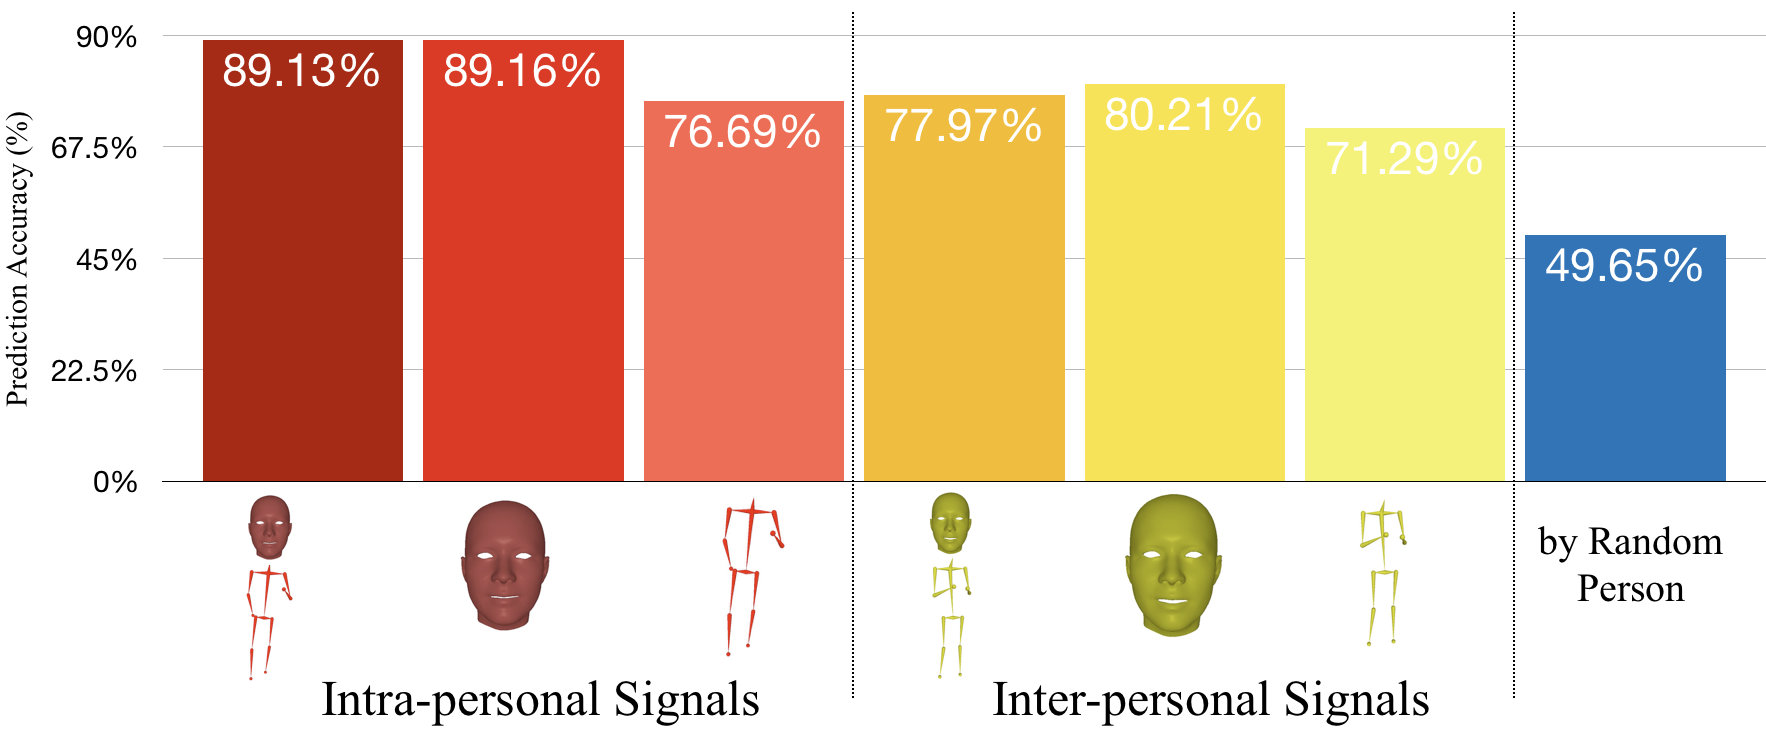
\includegraphics[ width=0.9\linewidth]{ssp_fig/result_speakPred_accuracy} 
%	\caption{Predicting Speaking Status} 
%	\label{fig:result_speakPred_accuracy}
%\end{figure}




% \begin{figure}
% 	\centering       
% 	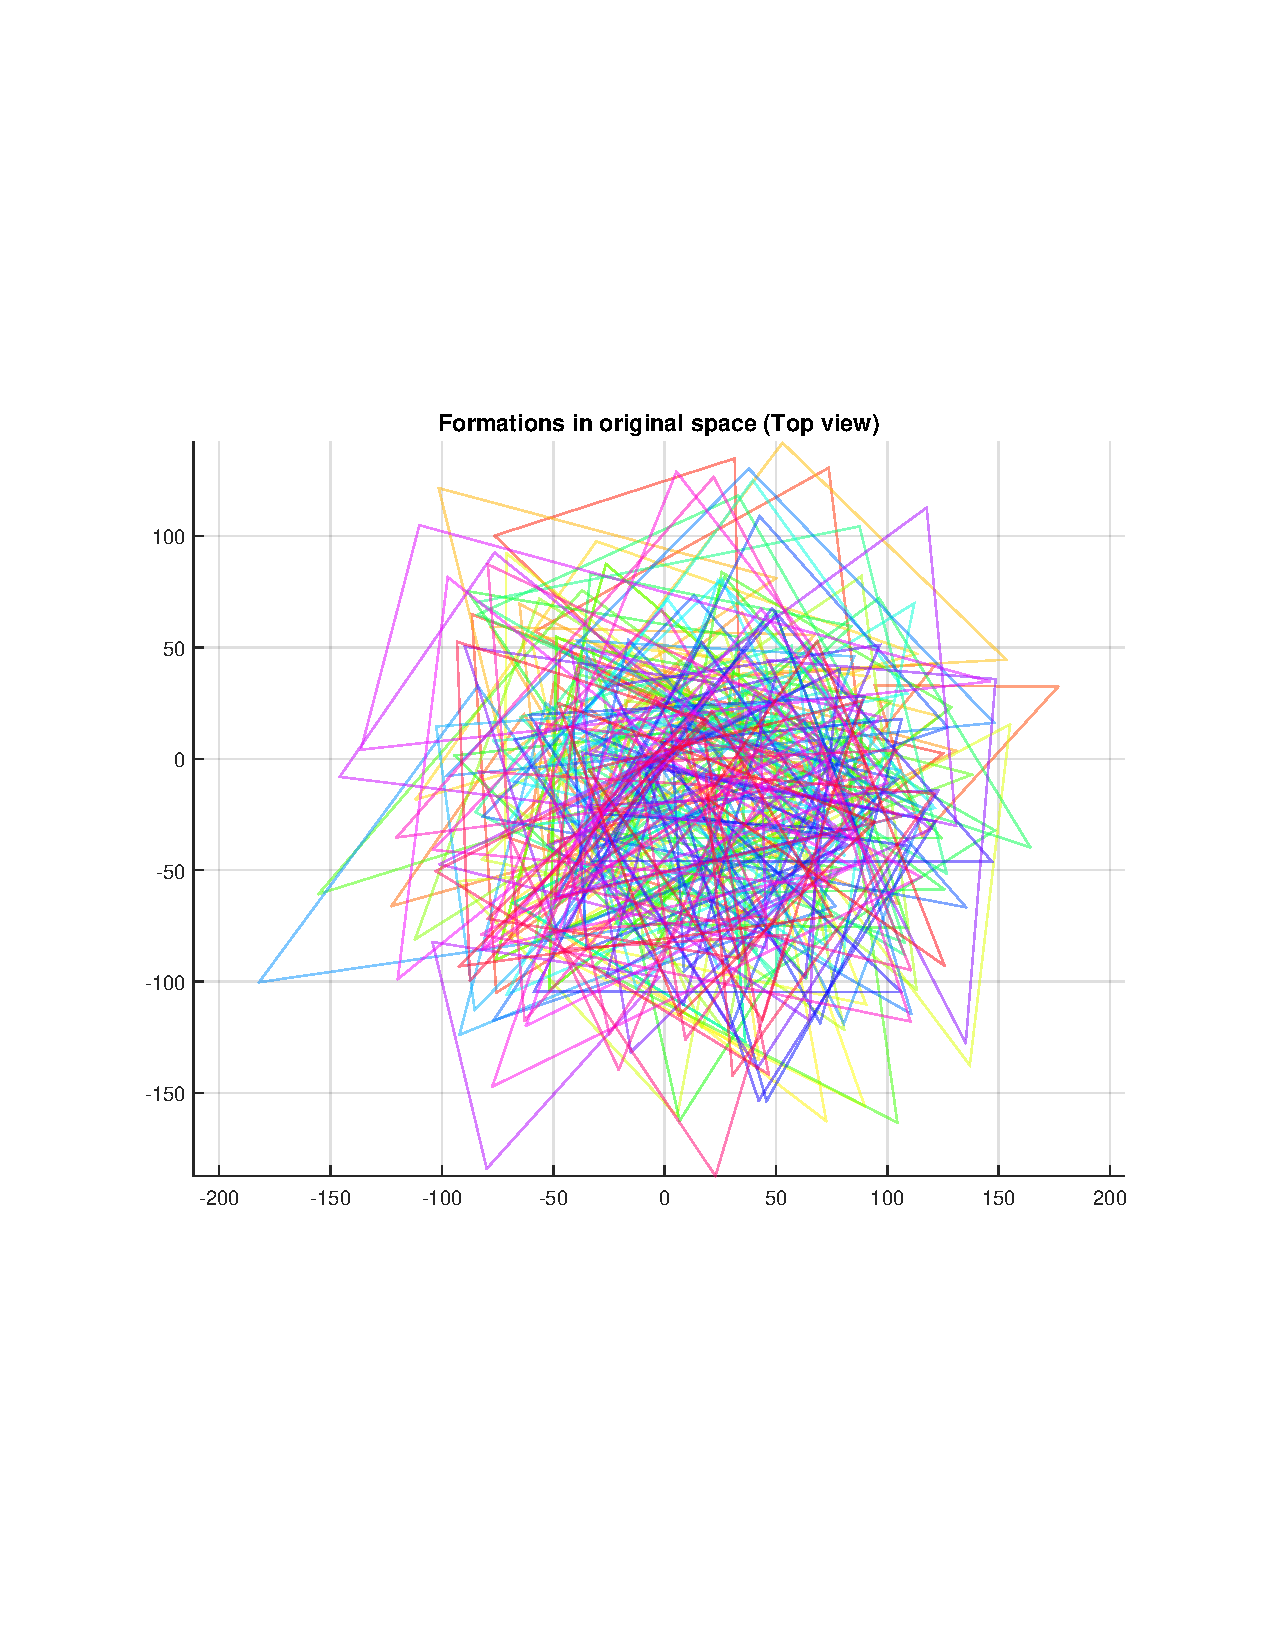
\includegraphics[trim=60 200 60 150,clip,width=0.32\linewidth]{fig/originalTri}
% 	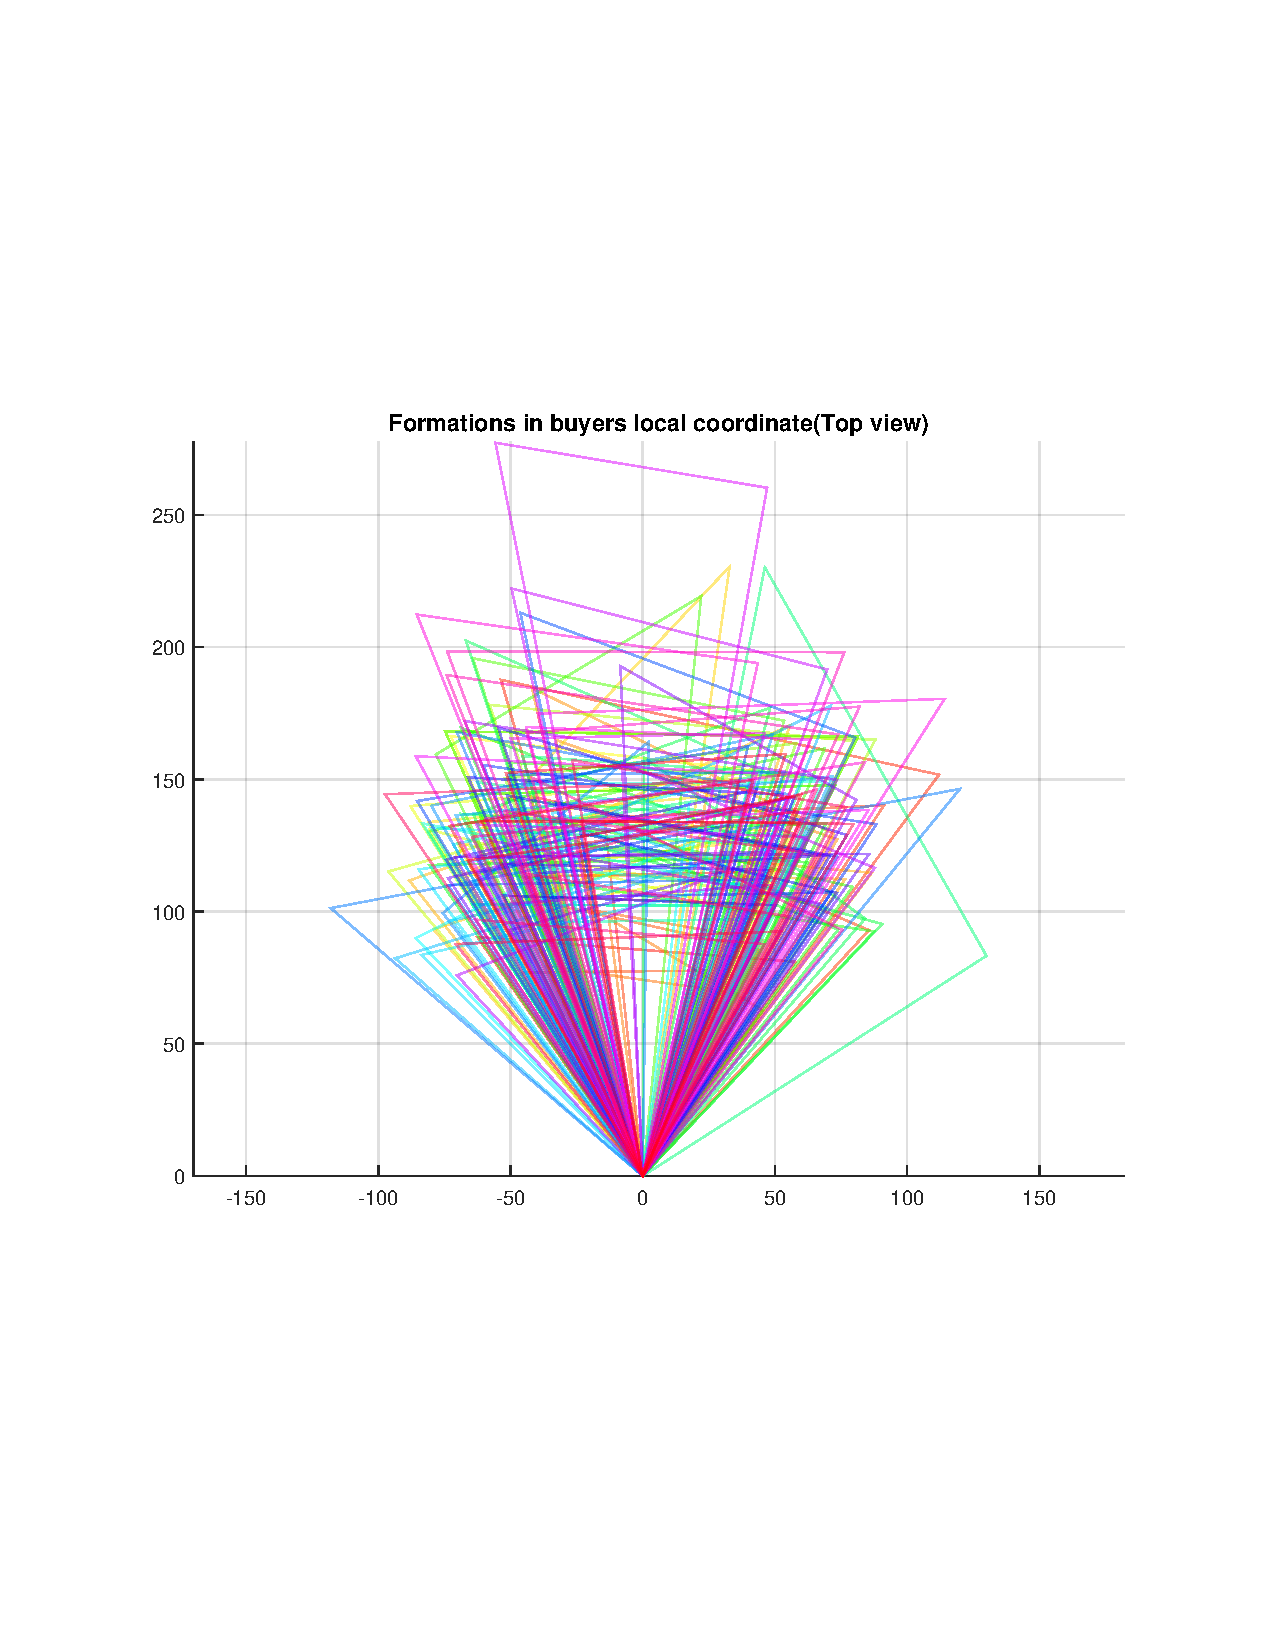
\includegraphics[trim=60 200 60 150,clip,width=0.32\linewidth]{fig/buyersTri} 
% 	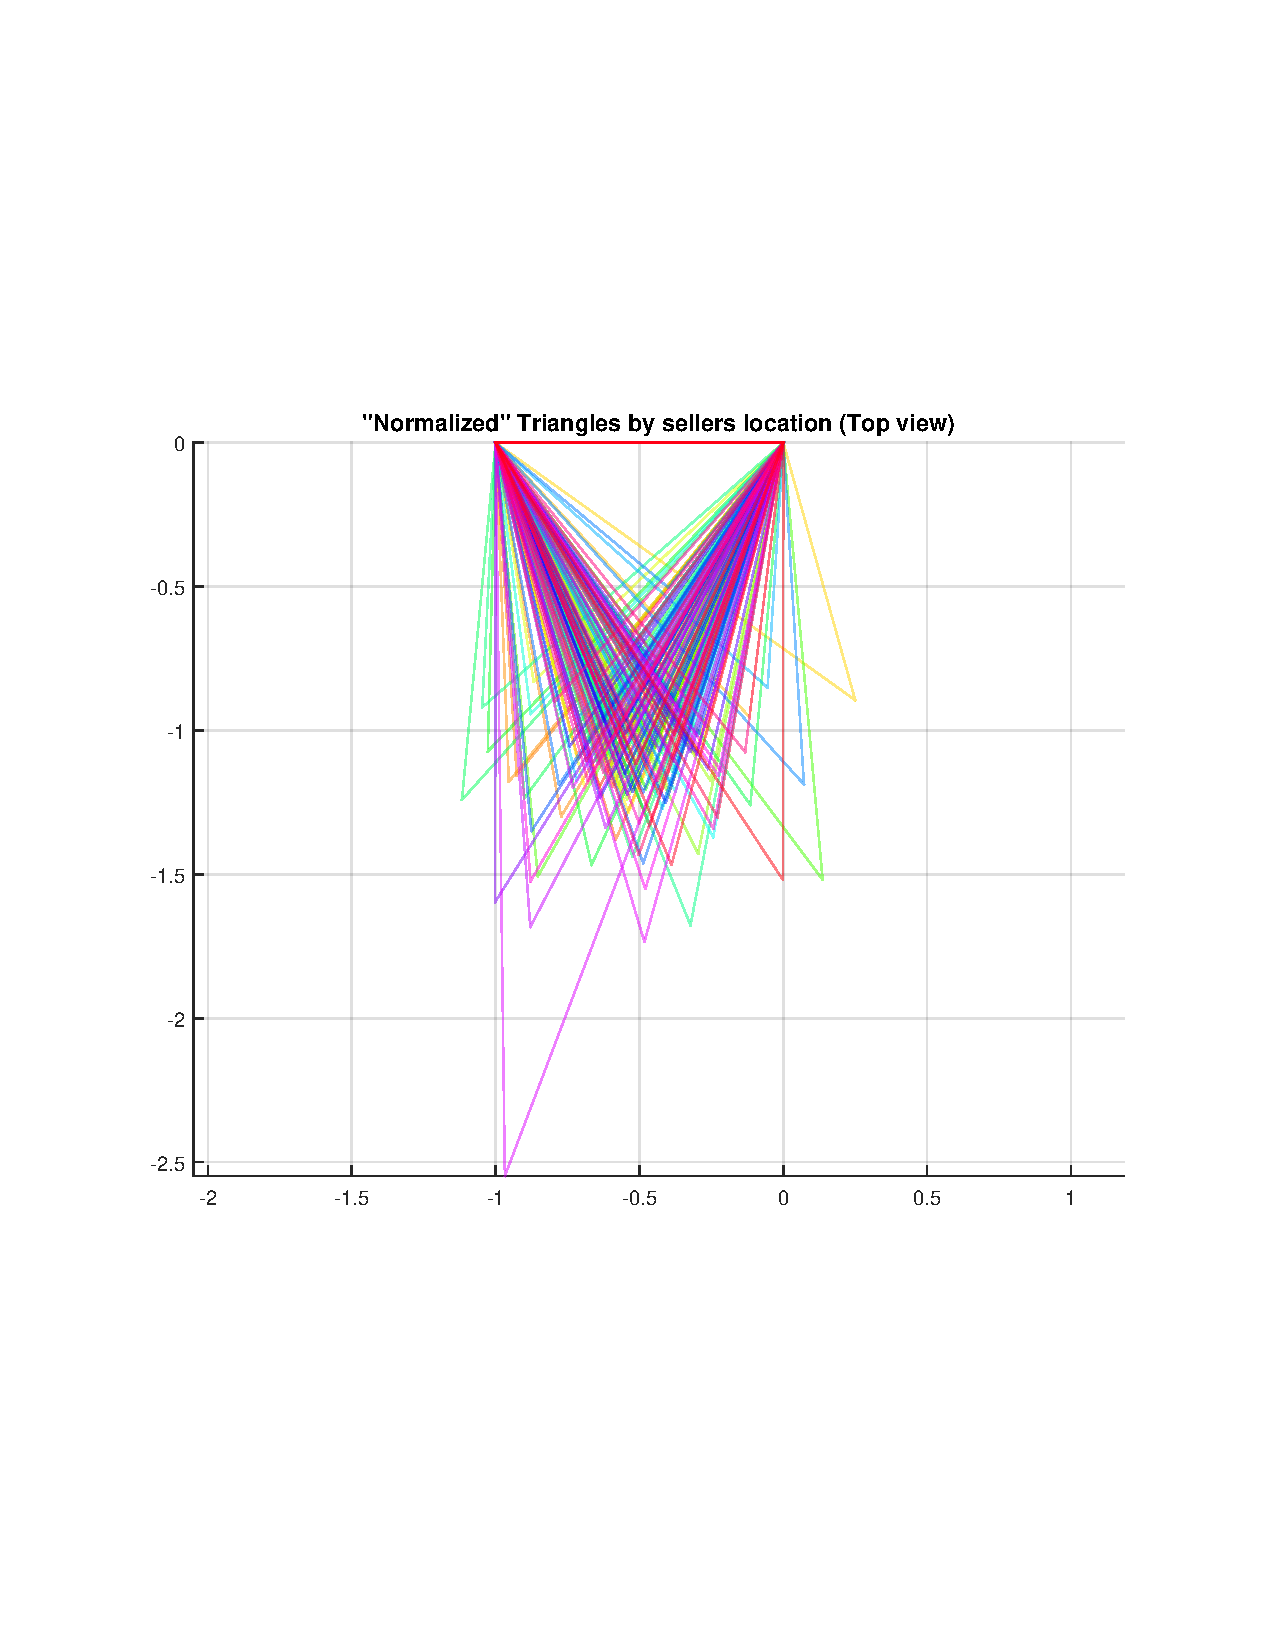
\includegraphics[trim=60 200 60 150,clip,width=0.32\linewidth]{fig/normTri} 
% 	%	\subfigure[TrajCompares]{\label{Fig:asso_traj}\includegraphics[width=0.5\textwidth]{img/trajCompare}}   
% 	\caption{Social formations in three different representations. (a) Global coordinate; (2) Person-centric coordinate defined by buyers; (3) Normalized-by-a-pair coordinate system define by two sellers} 
% 	\label{fig:socialgeo_distribution}
% \end{figure}



\subsection{Speaking Status Prediction}
We predict whether the target person is currently speaking or not by observing other channels of social signals in the scene.

\paragraph{A result on intra-personal signals.} First, we investigate the performance when the target individual's own social signals are used as input. Three different input sources--facial expressions, body gestures, and both of them---are used to train neural network models respectively. In particular, we use the same neural network architecture for this experiment by keeping the input dimension and network size as the same to make the comparison as fair as possible, as described in the method section. The prediction accuracies from these input signals are shown in the first column of Table ~\ref{table:speaking_class}. As demonstrated in our result, the social signals from the target individual show strong correlations with the speaking. For example, the facial cue of the target person shows the strongest correlation (about $90\%$ accuracy) with the target person's own speaking status, presumably due to the strong correlation between the lip motion and speaking. The body motion also shows a strong correlation with more than $76\%$ prediction accuracy. The result with both body and face signals, shown in the first column of Table ~\ref{table:speaking_class}, is similar to the case that only face cue is used, and by applying an ablation study we found that this is because the network dominantly uses the face cues over the body cues for the prediction, shown in the Table~\ref{table:speaking_class_ablation}. More specifically, given the trained model which takes both face and body as input, we mask out the face part or body part in the input data and compute their performances without any retraining. As shown in the Table~\ref{table:speaking_class_ablation}, the accuracy after removing the body part is similar to the original performance, while there exists much larger drop if the face part is removed. 


\begin{table}[t]
	\centering
	%	\footnotesize
	\begin{tabular}{c| c| c| c}
		\hline
		%Types & Avg. dist. (cm) & Std.(cm) & Min dist. (cm)  & Max dist. (cm)\\
		Input Signal Types/Sources & Self signal & Other seller's signal & Random person's signal\\
		\hline
		%Accuracy & 80.34\% & 73.44\% & 53.39\%\\
		%Accuracy & 76.16\% & 70.33\% & 51.05\%\\       %submitted
		Face+Body & 89.13\% & 77.97\% & 49.65\%\\       %new
		\hline
		Face & \underline {\textbf{89.16}}\% & \underline {\textbf{80.21}}\% & 49.64\%\\       %new
		\hline
		Body & 76.69\% & 71.29\% & 50.22\%\\       %new
		\hline
	\end{tabular}
	\caption{Speaking status classification accuracy using different social signal sources as input\label{table:speaking_class}}
\end{table}
\begin{table}[t]
	\centering
	%	\footnotesize
	\begin{tabular}{c| c| c }
		\hline
		%Types & Avg. dist. (cm) & Std.(cm) & Min dist. (cm)  & Max dist. (cm)\\
		Input Signal Types/Sources & Self signal & Other seller's signal \\
		\hline
		%Accuracy & 80.34\% & 73.44\% & 53.39\%\\
		%Accuracy & 76.16\% & 70.33\% & 51.05\%\\       %submitted
		Face+Body (original) & 89.13\% & 77.97\% \\       %new
		\hline
		After Removing Body & 85.11\% & 75.26 \% \\       %new
		\hline
		After Removing Face & 54.33\% & 67.64 \% \\       %new
		\hline
	\end{tabular}
	\caption{An ablation study after removing certain channels in the input for the networks trained with Face+Body input. The first row is the output of the original network (the same as in Table~\ref{table:speaking_class}), and next rows are testing performance after masking out body or face parts in the input data without any retraining. \label{table:speaking_class_ablation}}
\end{table}
\begin{figure}[t]
	\centering       
	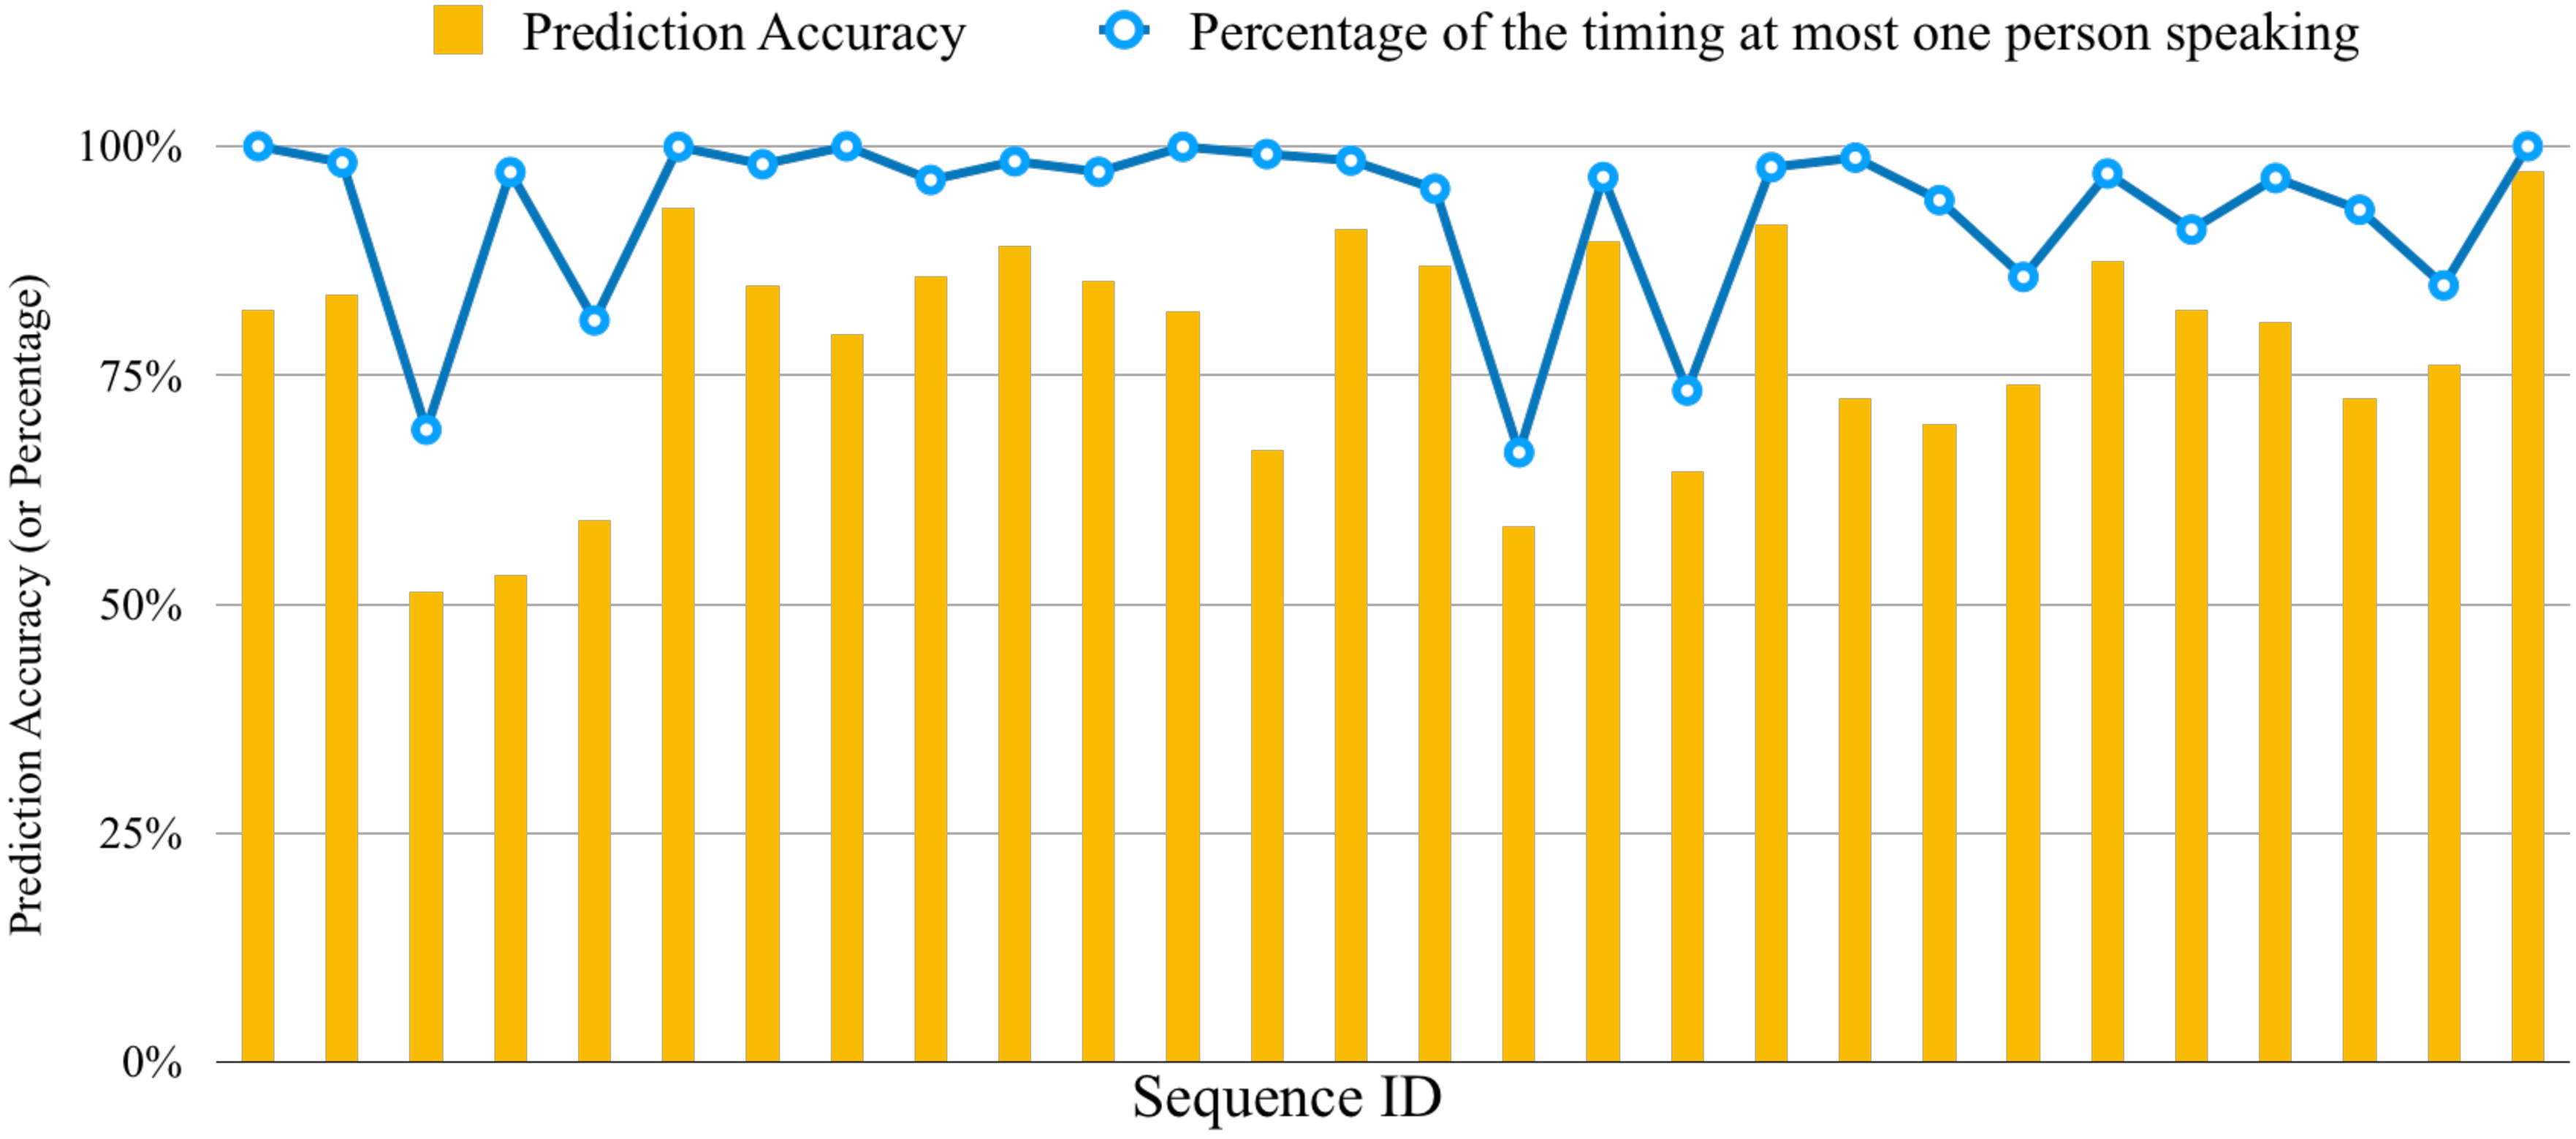
\includegraphics[ width=0.9\linewidth]{ssp_fig/turn-taking}
	\caption{Comparison between the performance of speaking status prediction and turn-taking status for each sequence. Each column shows the prediction performance (yellow bar) where the other seller's face and body signals are used as input. The blue curve represents how well the turn-taking rule is satisfied, which is defined by counting the percentage of the timing where at most one person is speaking. } 
	\label{fig:turn-taking}
\end{figure}
\begin{figure}[t]
	\centering       
	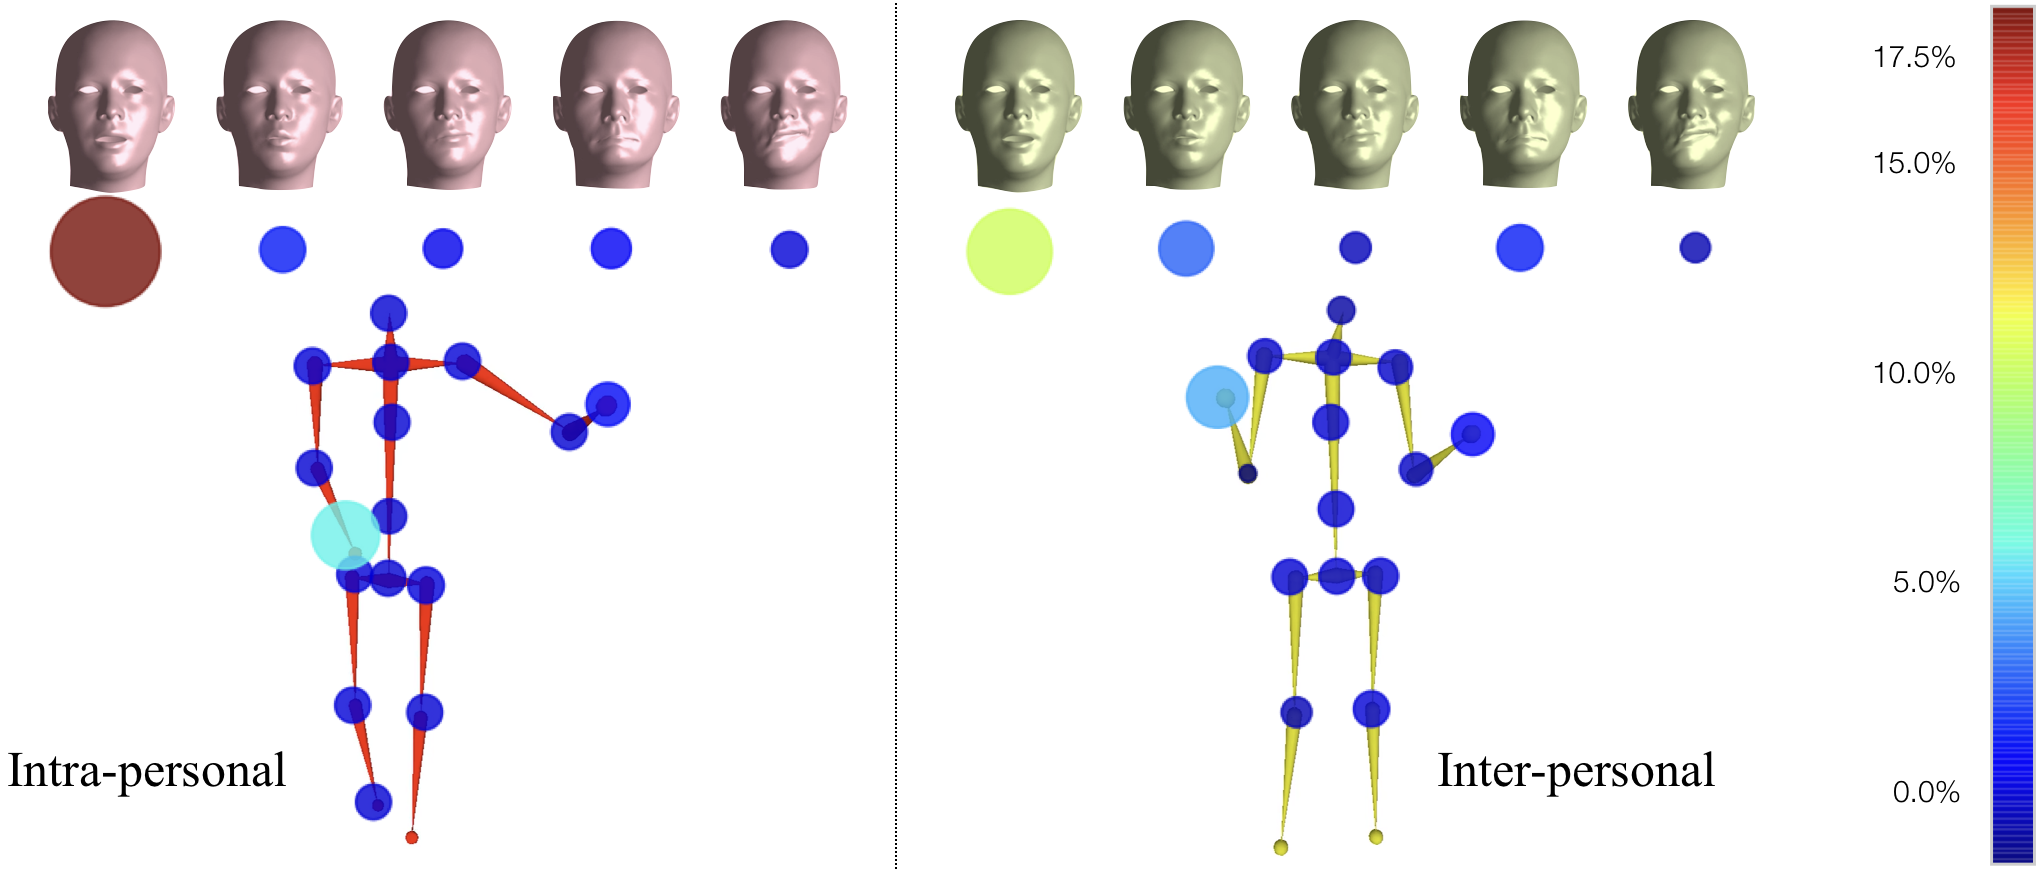
\includegraphics[ width=0.9\linewidth]{ssp_fig/result_speakPred_ablation}
	\caption{The result of an ablation study by comparing the prediction performances after removing each channel of the social signal input using the trained networks. We use the networks trained by using both body and face cues as input (the first row of the Table ~\ref{table:speaking_class}), and the performance drops after removing each part, compared to the original performances, are shown by colors and circle sizes. The left figure is the result by using the target person's own signals, and the right figure is by using the other seller's signals. The colorbar on the right shows the frame drops in percentage from the original performances.} 
	\label{fig:result_speakPred_ablation}
\end{figure}

\paragraph{A result on inter-personal signals.}
A more interesting experiment is investigating the performance by using the other seller's social signals as input to predict the target person's speaking status. Similarly, three different input sources are considered, and the results are shown in the second column of the Table ~\ref{table:speaking_class}.  The result clearly shows that there exists a strong link between interpersonal social signals. The other seller's facial motion shows a strong predictive power for the target person's speaking status, presumably due to the turn-taking property in social communication. For example, we can assume that the target person is not speaking, when the other seller is speaking. We can verify this by checking the tendency between the prediction performance and a measurement representing how well the turn-taking rule is satisfied during the communication, as shown in Figure~\ref{fig:turn-taking}. In this figure, we plot the speaking prediction accuracy for each testing sequence by using the other seller's both face and body signals as input, which is shown as yellow bars. The blue curve is the measurement to check the turn-taking status for each sequence, which is defined by counting the percentage of the timing where at most one person is speaking. In this measurement, 100\% means that there is no time that both sellers are speaking at the same time, where the turn-taking rules are perfectly satisfied. As shown in the figure, the prediction performance shows a very similar pattern to this turn-taking status. 

\paragraph{A result on random signals.}
As a comparison, we also perform the experiment using social signals from a random individual, where the individual is randomly selected in the testing set without any social link to our target individual. As shown in the third column of the Table~\ref{table:speaking_class_ablation}, the classification performance using a random person's motion as input shows about the chance level (50\%) with no predictive property.


\paragraph{An ablation study to verify the influence of each part.} As another test, we perform an ablation study by comparing the prediction performance after removing every single channel in the trained network. For this test, we use the network trained with both body and face cues (the first row of the Table ~\ref{table:speaking_class}). We mask out a certain channel (e.g., a face motion component or a body joint part) in the input and check the performance drop from the original output. The result is shown in Figure~\ref{fig:result_speakPred_ablation}, where the colors and the size of the circles represent the frame drops. This result shows that the first component of the face motion represents, which is corresponding to mouth opening motion, has the strongest predictive power for speaking status. As another interesting result, the result shows that the right hand has stronger predictive power than the left hand.  

%We compare the binary speaking classification performance . The task is to classify the speaking status of the target person, and we use three different body motion sources: (1) the target person's own body motion, (2) the other seller's body motion, (3) a random person's body motion. As shown in the results, the own body motion has the strongest correlation, but the other seller's body motion is also very predictive, showing that there exists a clear social link during their interaction. As expected, the classification performance using a random person's motion as input shows about the chance level (50\%). For the experiment (3), we use the same network trained for (2), but use the body motion from a subject in some other arbitrary sequence (excluding our current target sequence) as input. Presumably, the classification method using the other person's body signals learns the ``turn-taking" property in the social interaction, and predicts that the target person is speaking if little motion is observed from the other sellers (who would be listening). %This kind of study is important to make machines better understand human social behaviors, and can be facilitated from the data where natural social interactions are captured.  %This kin %shows an interesting insight that the body motions % the strong correlation of social signals can be used as a prior for predicting human behaviors. 
%\begin{table}[t]
%	\centering
%%	\footnotesize
%	\begin{tabular}{l| l| l| l}
%		\hline
%		%Types & Avg. dist. (cm) & Std.(cm) & Min dist. (cm)  & Max dist. (cm)\\
%		Input Signal & Own body & Other seller & Random person\\
%		\hline
%		%Accuracy & 80.34\% & 73.44\% & 53.39\%\\
%		%Accuracy & 76.16\% & 70.33\% & 51.05\%\\       %submitted
%		Accuracy & 80.70\% & 75.30\% & 51.05\%\\       %new
%		\hline
%	\end{tabular}
%	\caption{Speaking Classification Accuracy using different source of body motion signals as input\label{table:speaking_class}}
%\end{table}





\subsection{Social Formation Prediction (Position and Orientation)}
We predict the position and orientation of the target person, the ``left seller", by using the signals of communication partners. In this test, we explore the prediction accuracy by considering combinations of difference sources: using body position, body orientation, and face orientations. Table~\ref{table:predForm_errors} shows the results. By using all signals, we obtain the best performance. Intuitively, we can imagine that the target person's location can be estimated by triangulating the face normal direction of the other two subjects, which presumably learnt from our network. The prediction performance using only position cues shows the worst performance among them. 

We also introduce a baseline. The baseline method (denoted as ``Mirroring" in Table~\ref{table:predForm_errors}) predicts the location of the target seller to mirror that of the other seller w.r.t the buyer's body orientation, and estimate body orientation as the average between the two input subjects. The face orientation is chosen to always face the buyer. This baseline has large errors, with poor prediction results when the buyer is directly facing the other sellers, making the target person be too close to the other seller. 



\begin{table}[t]
	\centering
	%	\small
	%\caption{Social Formation Prediction Errors (cm) }
	\begin{tabular}{c| c| c| c}
		\hline
		%Types & Avg. dist. (cm) & Std.(cm) & Min dist. (cm)  & Max dist. (cm)\\
		Types & Position & Body Orientation & Face Orientation\\
		\hline
		PosOnly & 29.83 (13.38) & 0.26 (0.12) & 0.33 (0.13) \\
		\hline
		Pos+face & 25.23 (9.74) & 0.23 (0.09) & 0.30 (0.12) \\
		\hline
		Pos+body & 26.57 (10.24) & 0.22 (0.08) & 0.30 (0.10) \\
		\hline
		Pose+face+body & \underline {\textbf{24.59}} (10.23) &  \underline {\textbf{0.21}} (0.06) &  \underline {\textbf{0.29}} (0.09) \\
		\hline
		Mirroring (baseline) &  50.03 (20.84) & 0.40 (0.17) & 0.52 (0.14) \\
		\hline
	\end{tabular}
	\caption{Social Formation Prediction Errors (cm). Average position error between our estimation and ground-truth are reported in centimeters. The body orientation and face orientation are computed between the distance of estimated facial/body normal direction and GTs.\label{table:predForm_errors}}
\end{table}


%Our method shows a 25 cm error in the prediction, which is better than a baseline. As the baseline, we predict the location of the target seller to mirror that of the other seller w.r.t the buyer's body orientation, and estimate body orientation as the average between the two input subjects. The face orientation is chosen to always face the buyer (denoted as ``Mirroring" in Table~\ref{table:predForm_errors}). We also perform an ablation study to see what information is important to get better accuracy. To do this, we change the channel of the input, as in Table~\ref{table:predForm_errors}. We use the same network  but set unused input channels to their mean values in the training set. This experiment demonstrates that social formation estimation can take advantages from the body and face orientation signals. Intuitively, we can imagine that the target person's location can be estimated by triangulating the face normal direction of the other two subjects. To compute errors of orientations, we compute the 2D distance between the unit vectors representing the orientation estimation and the ground truth normal directions of face or body.% In Fig.~\ref{fig:predForm_errors}, the average position errors of each sequences are shown. 

%\begin{figure}
%	\centering
%	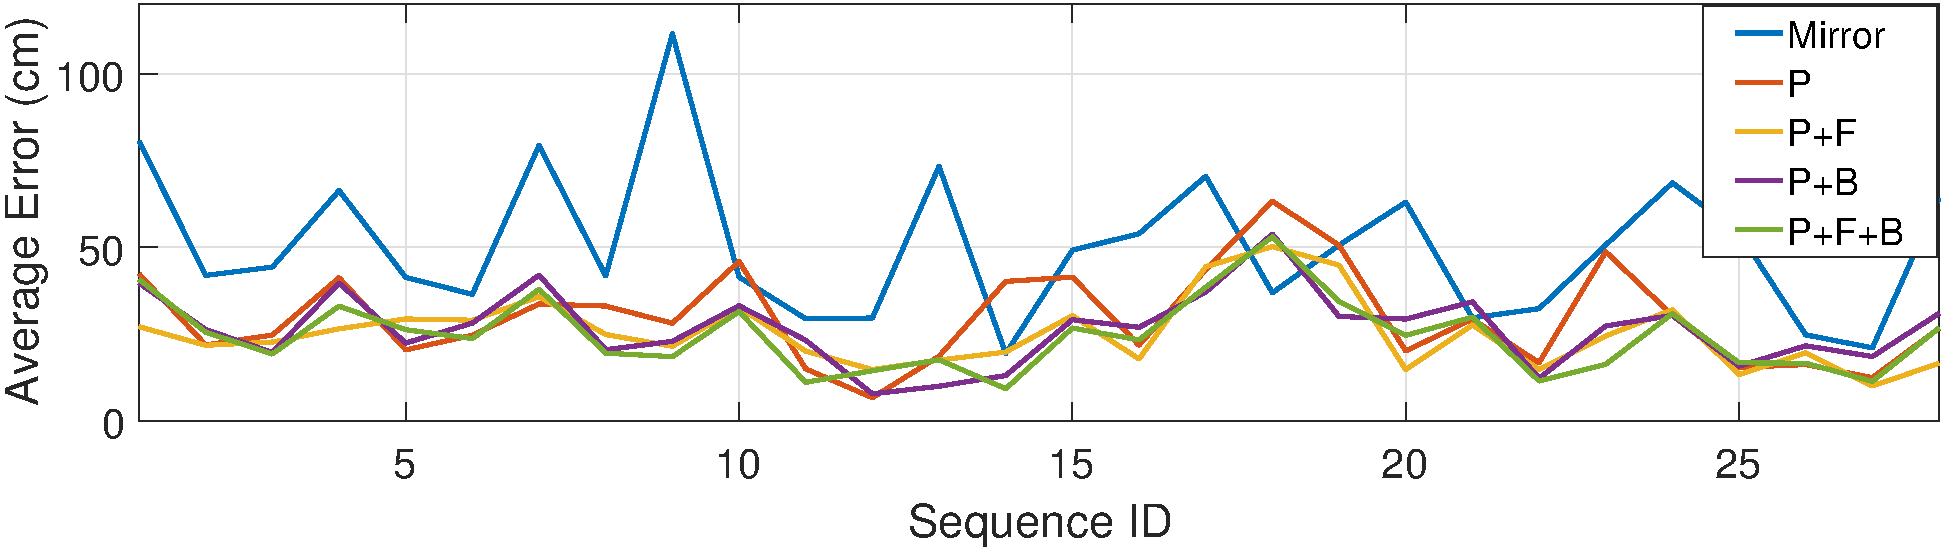
\includegraphics[width=\linewidth]{ssp_fig/cvpr19_predForm}\\
%	\includegraphics[width=\linewidth]{ssp_fig/cvpr19_predBody}
%	\caption{Average error of social formation prediction (top) and body gesture prediction (bottom). $y$-axis for the position errors in centimeters, and $x$-axis is sequence IDs.} %``Mirror" represents the baseline method, and P, F, and B denote Position, Face orientation, and Body orientation, as the input for the prediction.} 
%	\label{fig:predForm_errors}
%\end{figure}



% %Body only
% total_avg_posErr: 29.8286890398, std 13.3812589645
% total_avg_bodyOriErr: 0.263378293988, std 0.124290071428
% total_avg_faceOriErr: 0.327747834313, std 0.129691809416

% %Body + face
% total_avg_posErr: 25.2330815723, std 9.74251270294
% total_avg_bodyOriErr: 0.228412316901, std 0.0890485420823
% total_avg_faceOriErr: 0.303724261948, std 0.116639345884

% %Body + bodyOri
% total_avg_posErr: 26.57, std 10.24
% total_avg_bodyOriErr: 0.22, std 0.08
% total_avg_faceOriErr: 0.30, std 0.10

%While lower error may mean a better result, we may still see whether the prediction behave as human. 
% {\color{red} What happen when the turns are changing }

% {\color{red} Failure cases?}

% Position only, and orientation. 

% W/Wo speaking

% W/Wo body signal

% PCK curves

% Baseline: Trianglular estimation
% Orientation: See always the buyer.

% \begin{figure}
% 	\centering
% 	\includegraphics[width=\linewidth]{plot/cvpr19_predBody}
% 	\caption{Average error of body prediction. $y$-axis for the errors in centimeter, and $x$-axis for the sequences.} 
% 	\label{fig:predBody_errors}
% \end{figure}

%\begin{figure*}
%	\centering       
%	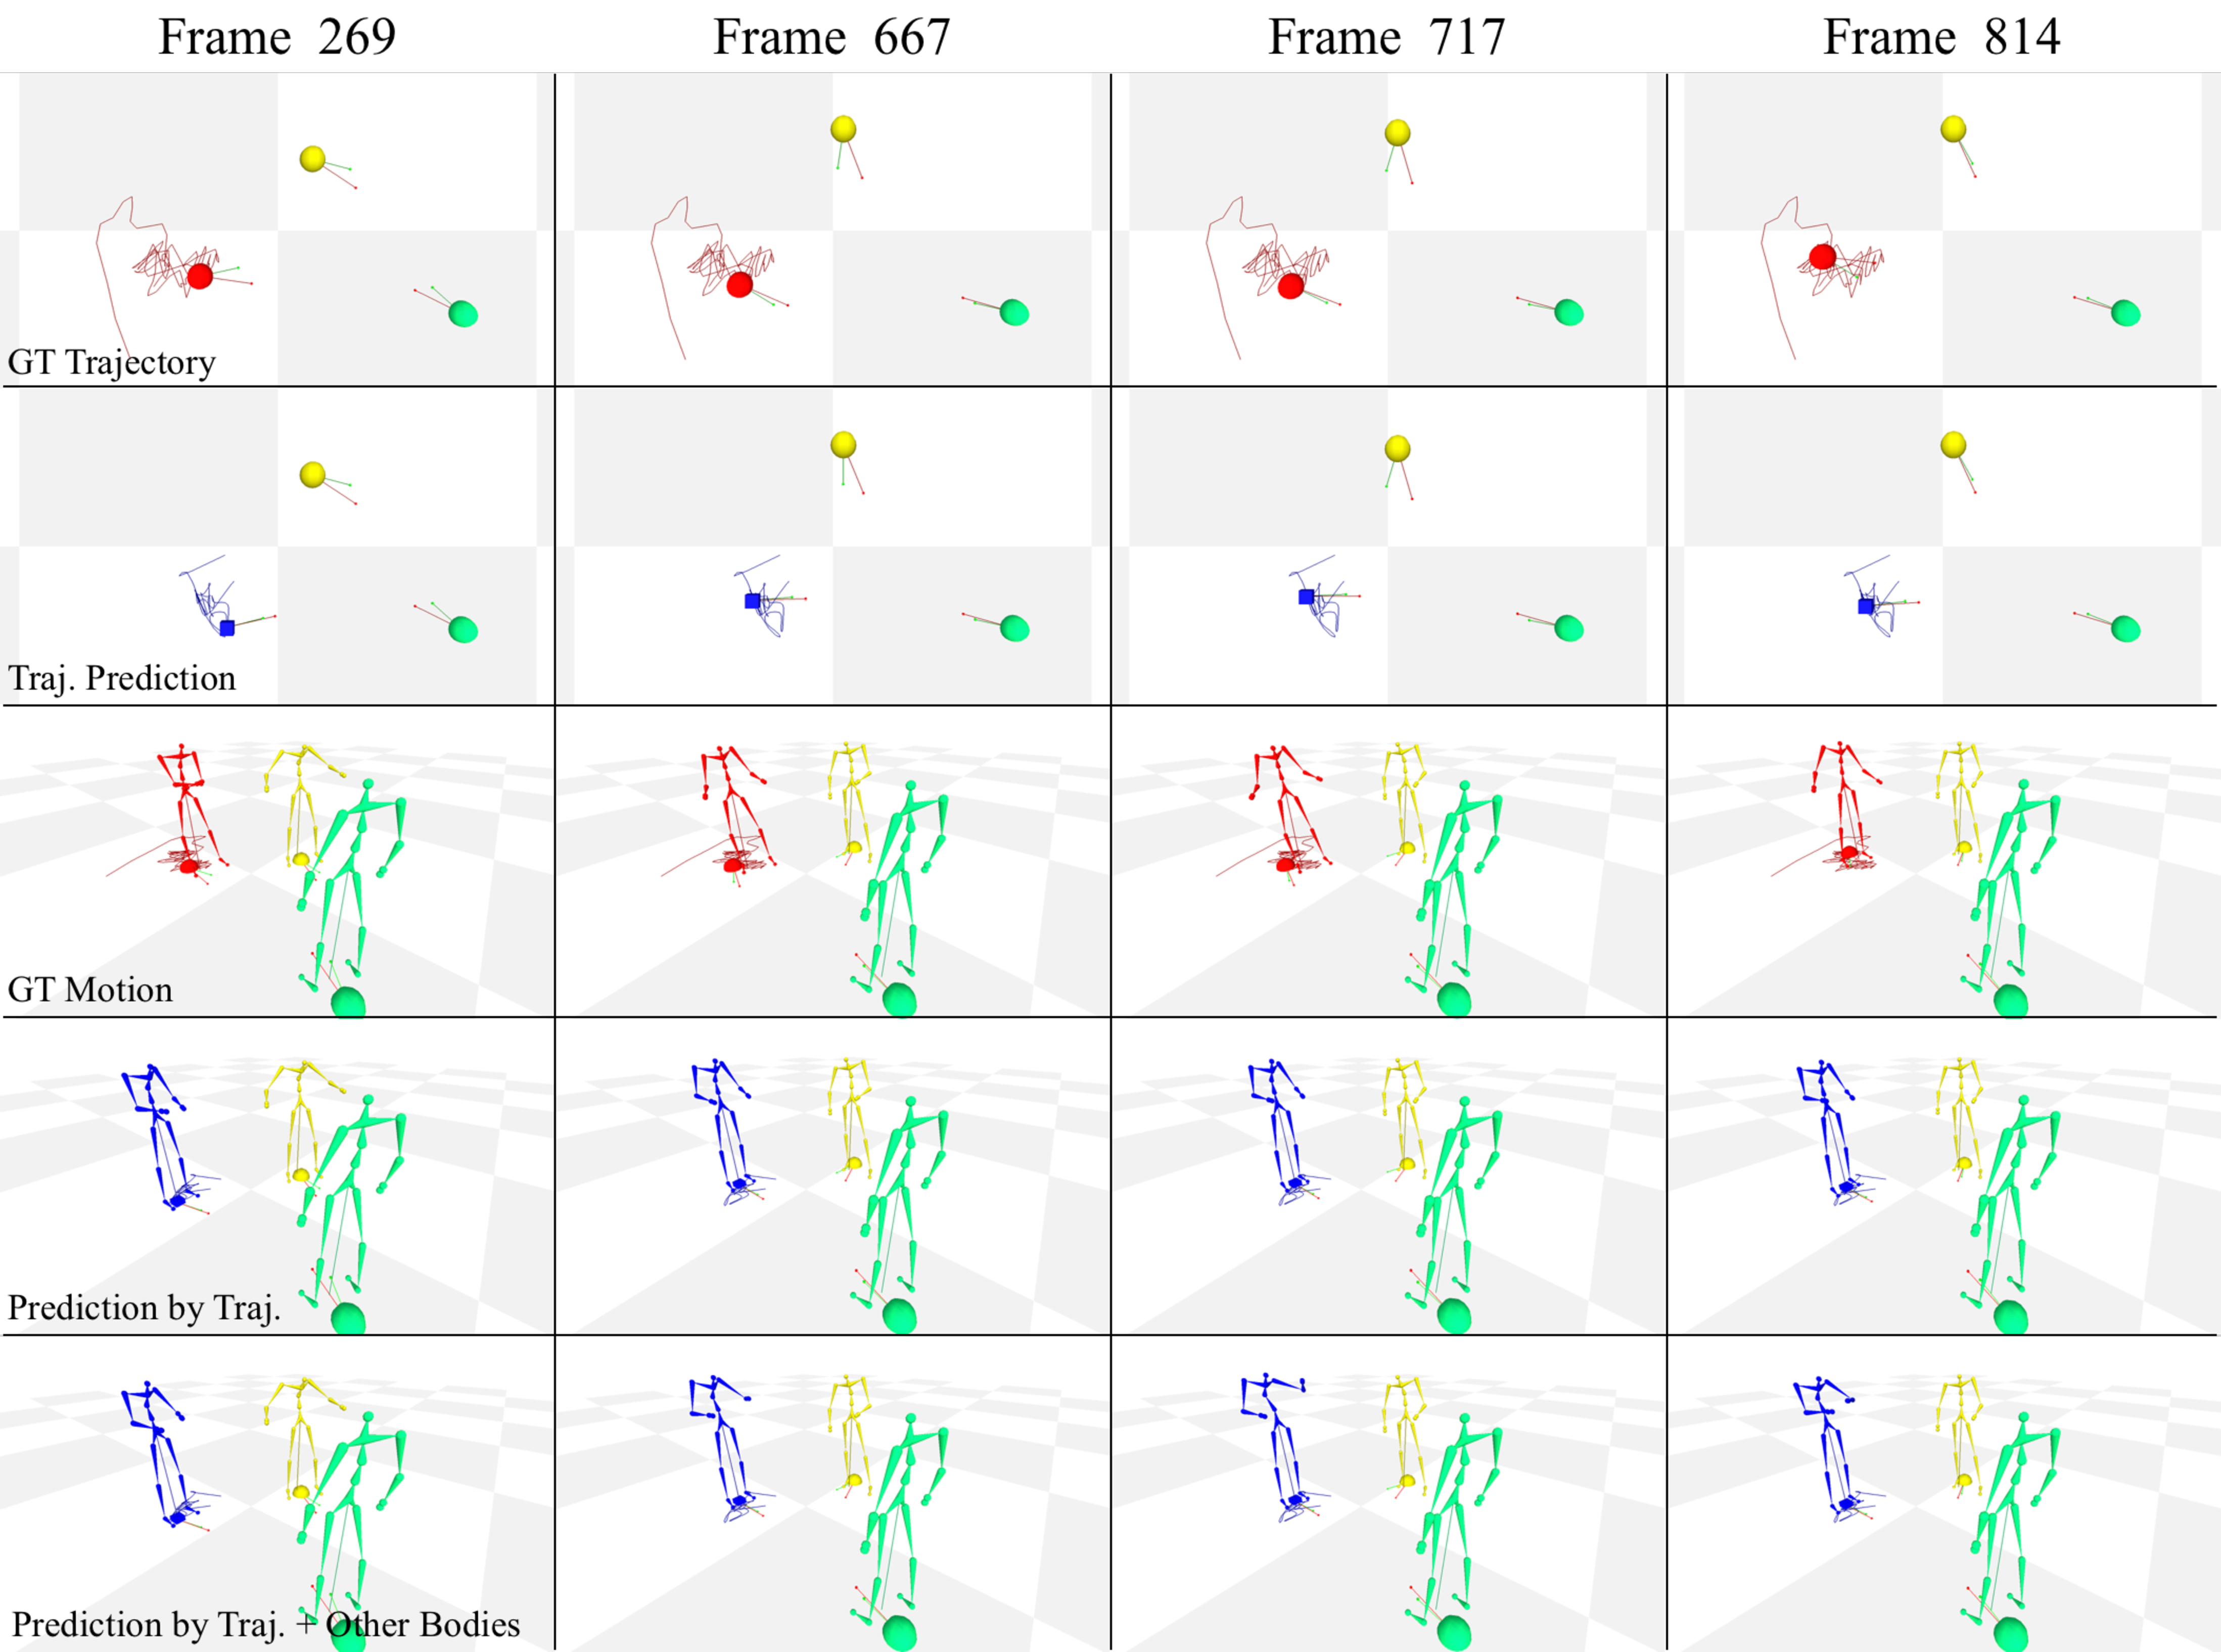
\includegraphics[width=\linewidth]{ssp_fig/qual_170221_b2_group4}
%	%	\subfigure[TrajCompares]{\label{Fig:asso_traj}\includegraphics[width=0.5\textwidth]{img/trajCompare}}   
%	\caption{An example result of \textit{Social Signal Prediction}. Each column shows scenes at a particular frame. The social signals drawn in green or yellow color are used as the inputs to our method, and blue signals are our social signal prediction results. The signals drawn in red are the ground truth. (First row) The ground truth social formations are shown from a top view, where the target person is shown as red spheres along with trajectories (red curves), face orientation (green arrows pointing from the spheres), and body orientations (red arrows from the spheres). (Second Row) The predicted locations (blue cubes), trajectories (blue curves), face orientations (green arrows), and body orientations (red arrows) are shown. (Third row) The ground-truth 3D body poses of the target person are shown. (Fourth row) We predict the 3D motion from the estimated 2D trajectory of the target person. (Fifth row) We use the body motion of other subjects to predict the upper body motion of the target person, which are combined to the leg body motions estimated from the trajectories.} 
%	\label{fig:qualitative}
%\end{figure*}


\subsection{Revisiting Proxemics}
An interesting experiment is to consider the well-know theories in psychology again using the new data we collected in our sensor system. Our dataset has the measurement of fully spontaneous motions (including the position and orientation of groups) of interacting people, and enables us to revisit the well-known proxemics theory~\cite{Hall66}. We first compute the average distance between a pair of subjects: (1) buyer and right sellers (B-RS), (2) buyer and left seller (B-LS), and (3) left seller and right seller (LS-RS). The results are shown in Table~\ref{table:proxemics_comp}. We found that the result approximately follows the social distance categories defined in the Hall's categorization~\cite{Hall66}. The distances among sellers are within the close phase of social distance ranges (from 120-210 $cm$) and the average distance among sellers and buyers are within the far phase of social distance (from 210 to 370 $cm$) in \cite{Hall66}. To analyze the shape of the social formation, we plot the average formation of games in a person-centric coordinate by a buyer. The results are shown in the Figure~\ref{fig:socialgeo_distribution}, showing that the formation is often similar to isosceles triangles with relatively far distances between a buyer and two sellers than the distance between sellers. 


\begin{figure}
	\centering       
	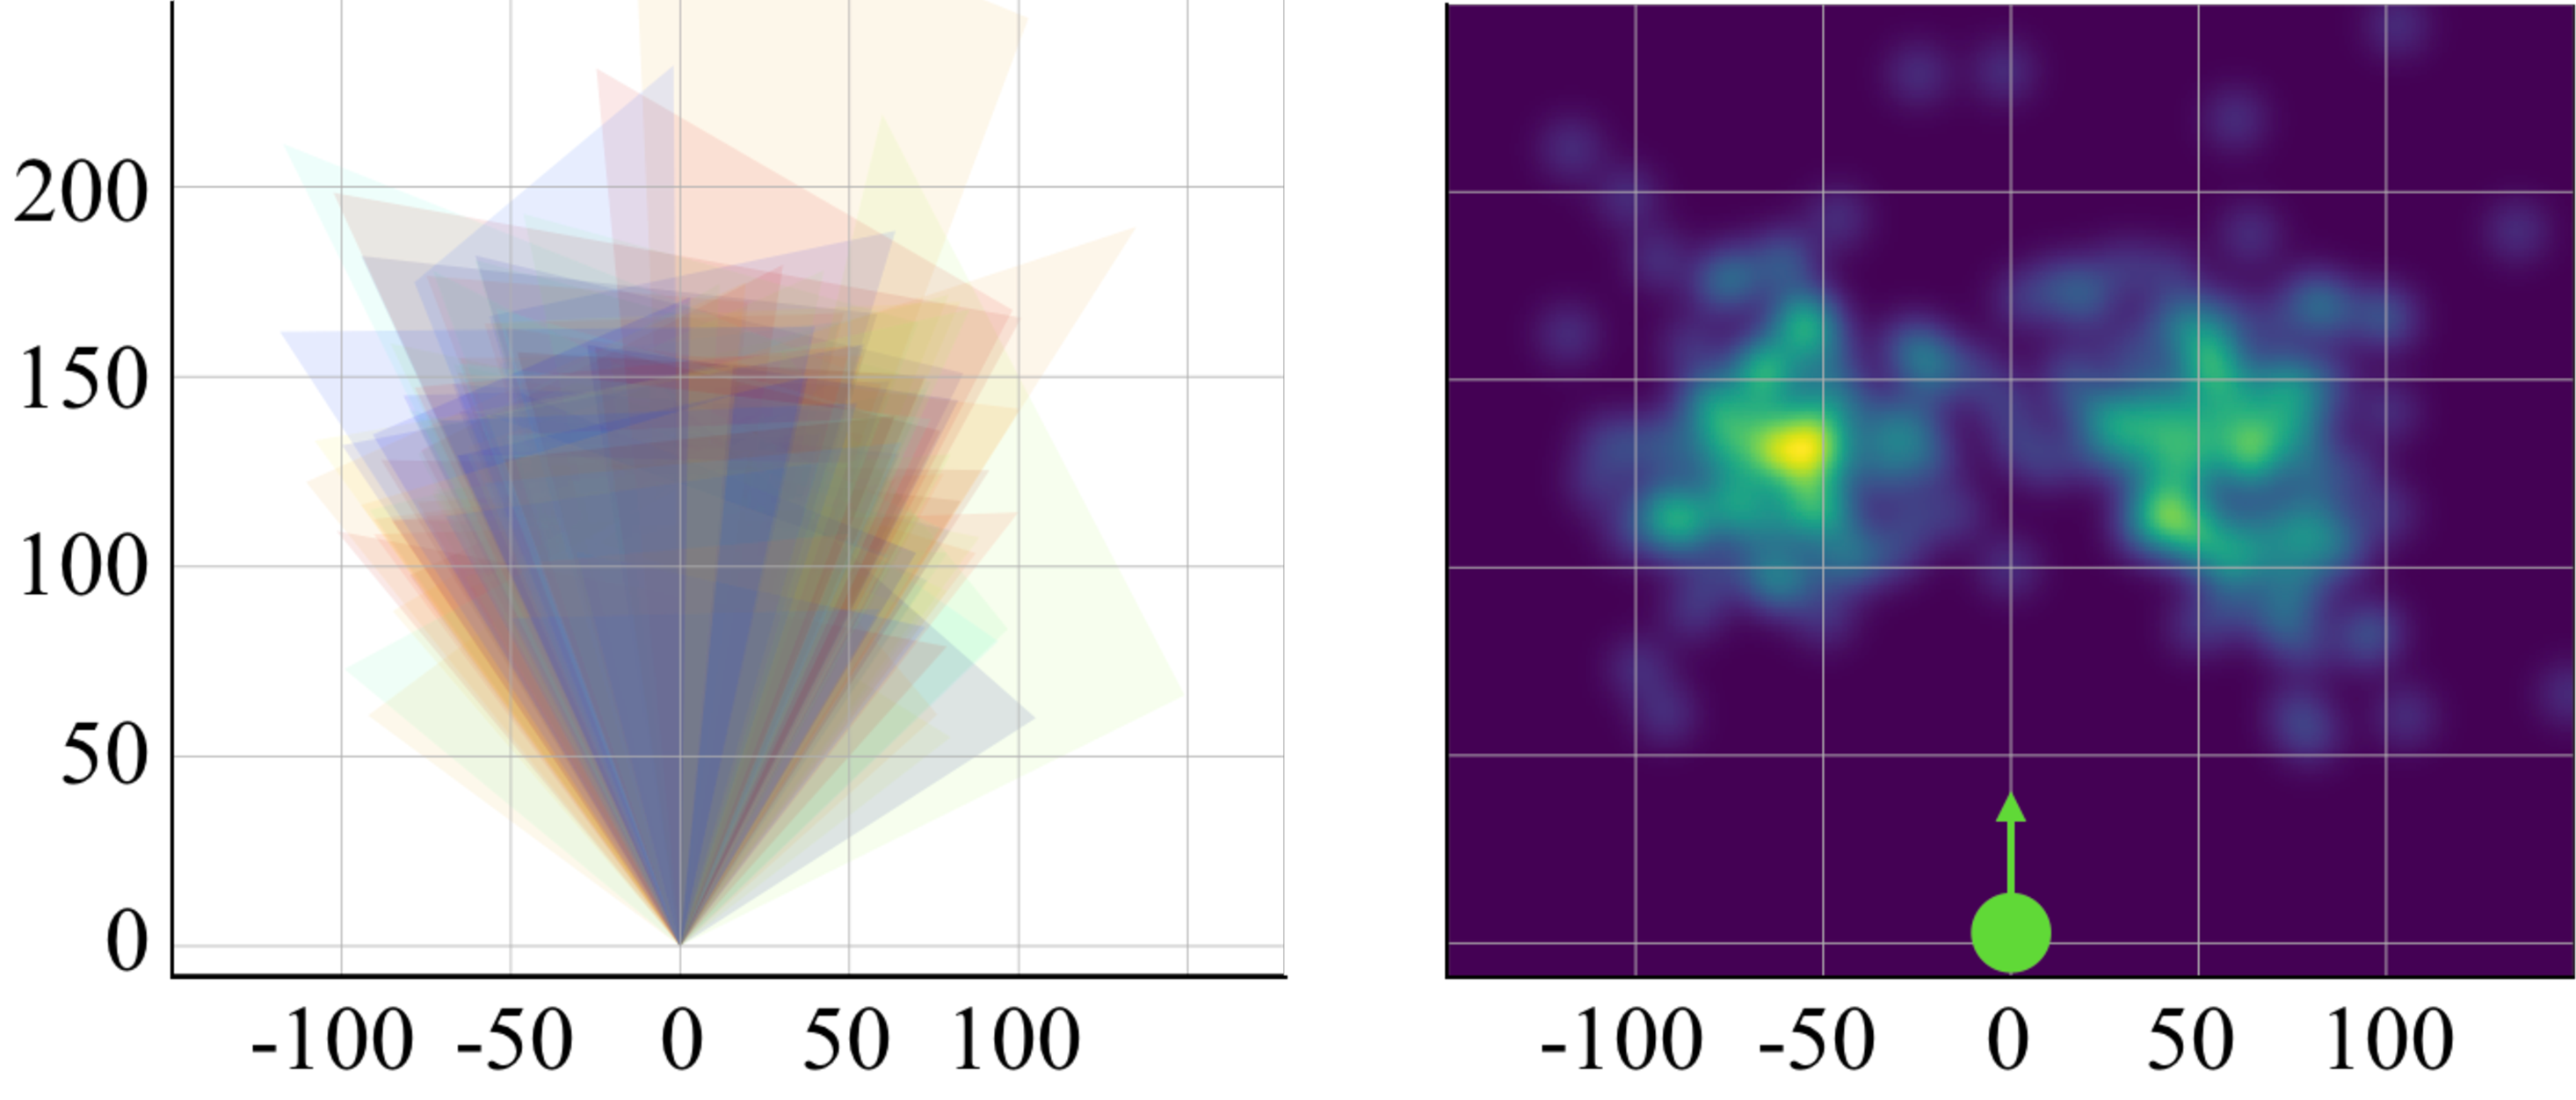
\includegraphics[ width=0.8\linewidth]{ssp_fig/haggling_proxemics_stat.pdf}
	% 	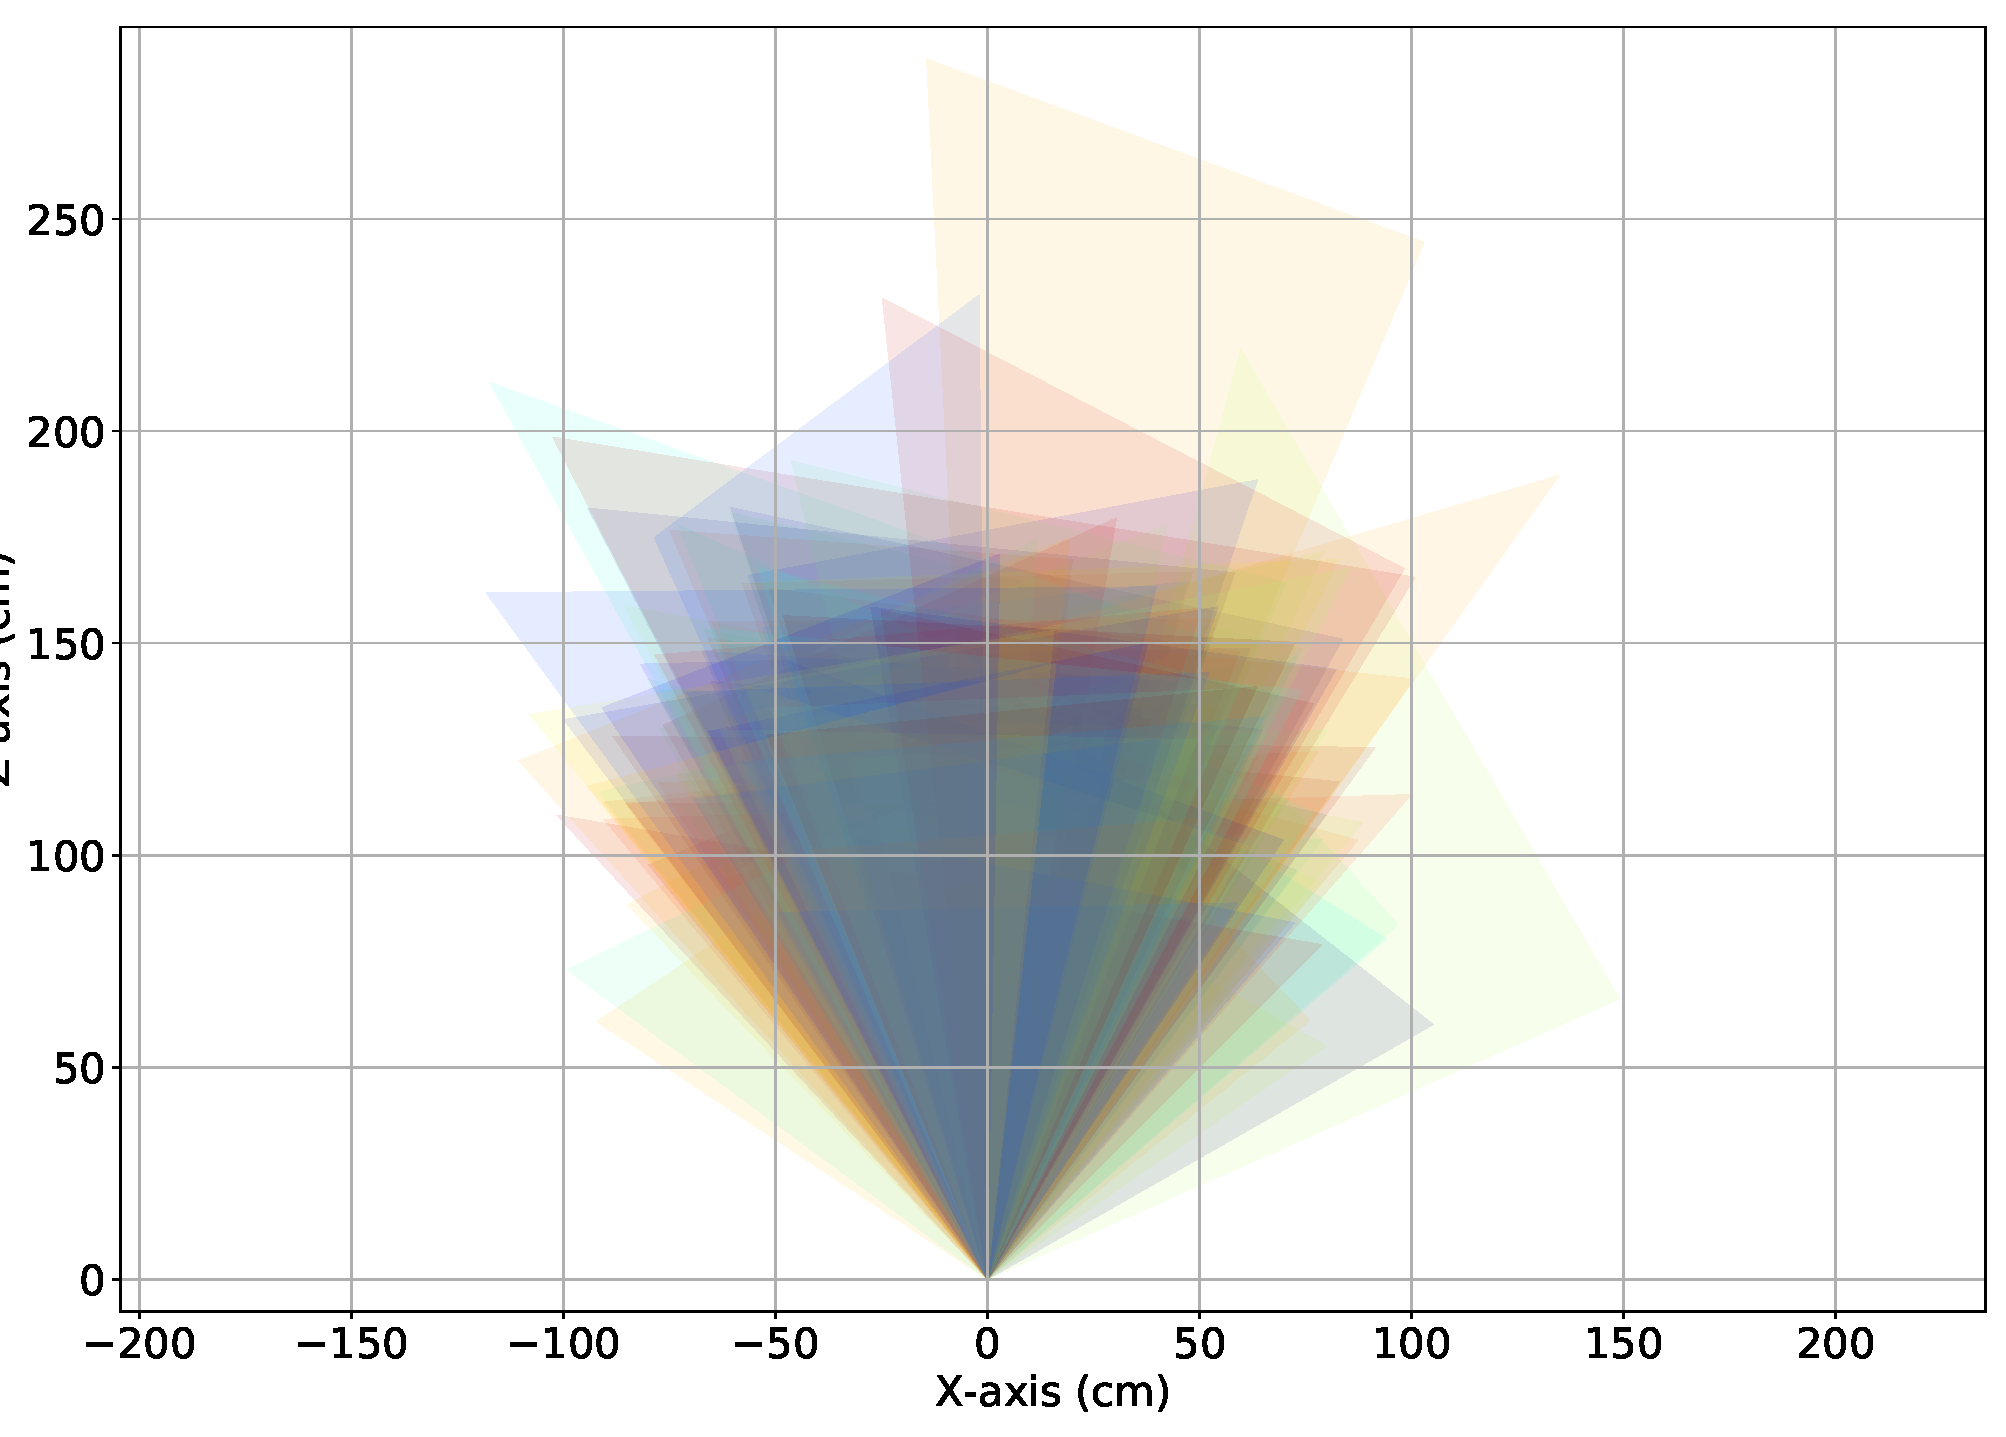
\includegraphics[trim=120 0 120 0,clip, width=0.45\linewidth]{plot/haggling_proxemics_polygon.pdf}
	% 	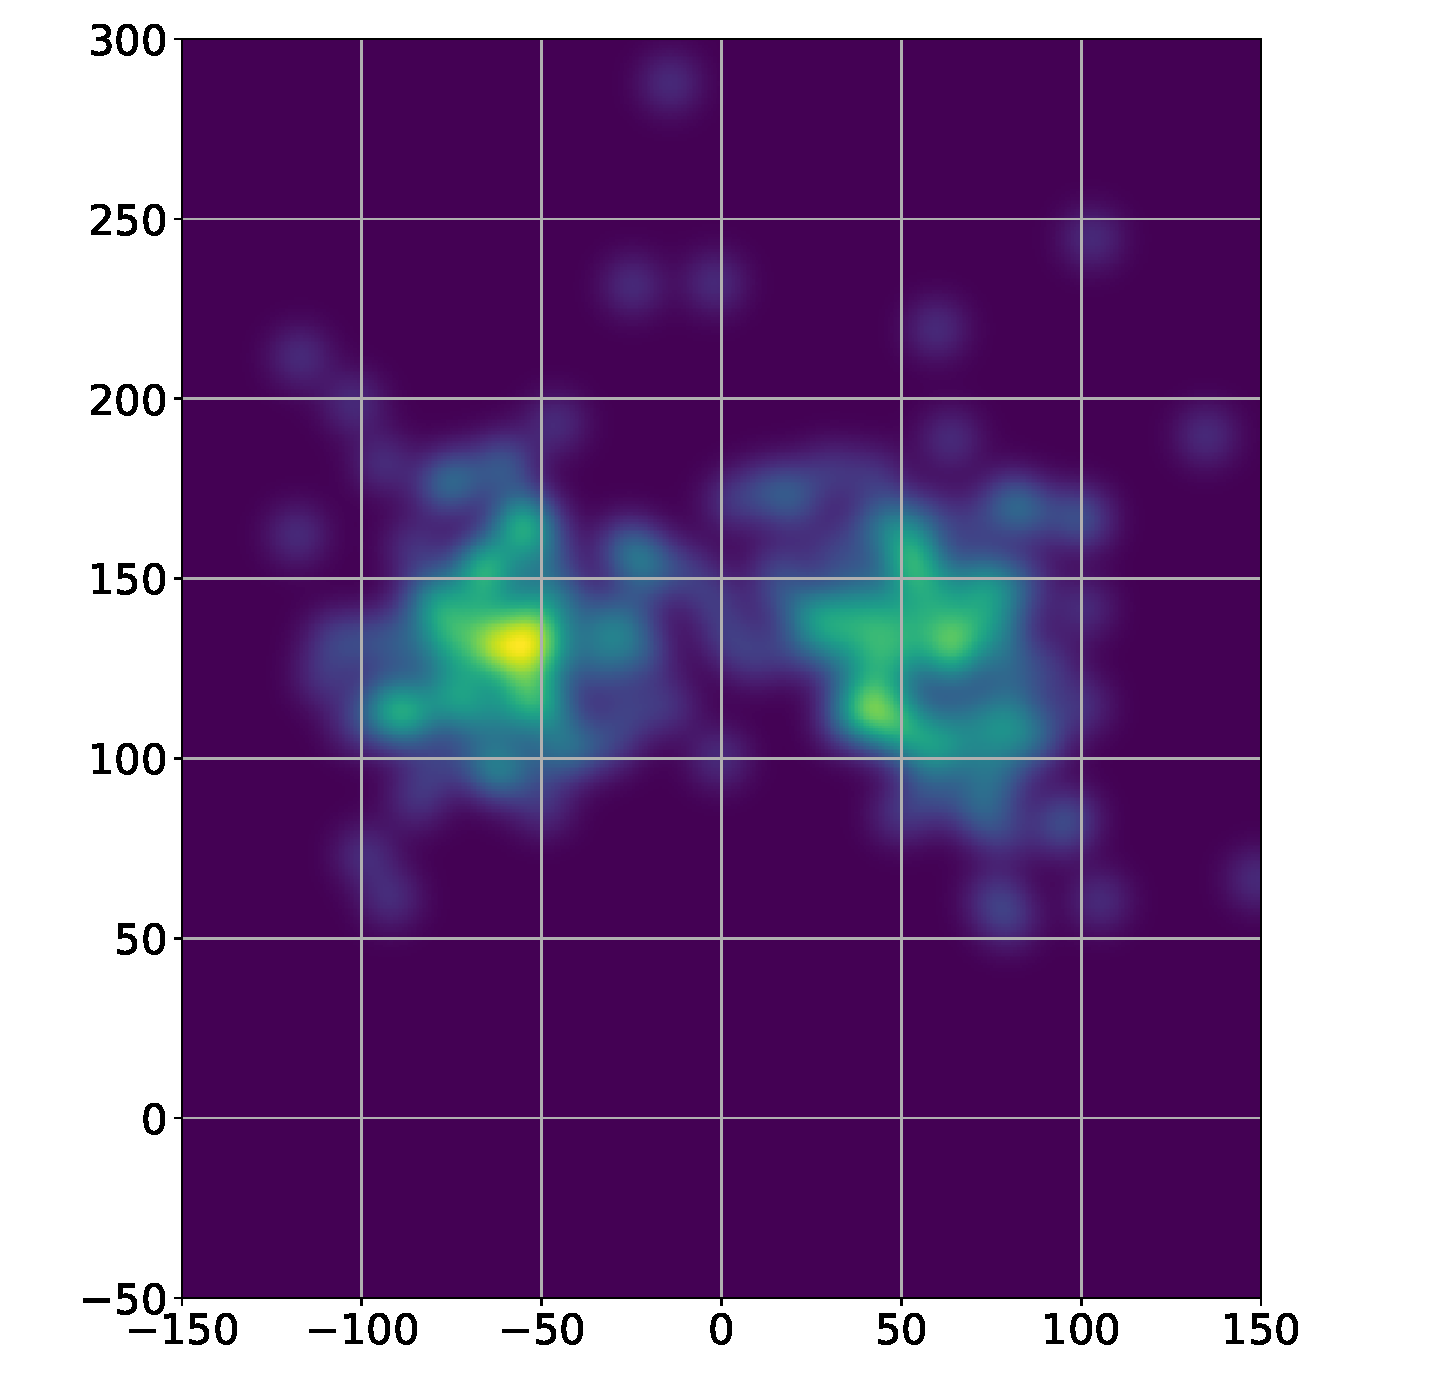
\includegraphics[width=0.45\linewidth]{plot/haggling_proxemics_heatmap.pdf} 
	%	\subfigure[TrajCompares]{\label{Fig:asso_traj}\includegraphics[width=0.5\textwidth]{img/trajCompare}}   
	\caption{Visualizing social formations in the haggling sequences as triangles (left) and a heat map (right). The formation is normalized w.r.t the buyer's location, and the green circle on the right shows the buyer location (origin) and orientation ($z$-axis).} 
	\label{fig:socialgeo_distribution}
\end{figure}




\begin{table}[t]
	\centering
	%	\footnotesize
	\begin{tabular}{c| c| c| c| c}
		\hline
		%Types & Avg. dist. (cm) & Std.(cm) & Min dist. (cm)  & Max dist. (cm)\\
		& Avg. dist. & Std. & Min & Max \\
		\hline
		B-RS & 148.11 & 27.26 & 99.03 & 265.52 \\
		\hline
		B-LS & 151.45 & 29.62 & 104.24  & 284.85 \\
		\hline
		LS-RS & 124.13 & 24.05  & 77.70  & 206.26 \\
		\hline
	\end{tabular}
	\caption{Average distances (cm) between subjects. B, RS, and LS denote buyer, right seller, and left seller respectively.}
	\label{table:proxemics_comp}
\end{table}

\subsection{Verifying The Bias of Buyer's Body Orientation Toward Winner}
As results of haggling games, the decisions of buyers are known, making winners and losers between two sellers. Equipped with the body location and orientation measurements of all individuals, we can quantitatively verify whether there exists any bias in the body orientations of buyers toward winners. To check this, we first normalize the orientation cues of the buyers with respect to both sellers as shown on the right of the Figure~\ref{fig:result_buyer_bias}, where the orientation of a buyer with respect to two sellers is represented by a value around $0.0$ and $1.0$ at a time. In this representation, $0.0$ means that the buyer's body is fully facing the winner, and $1.0$ means that buyer's body orientation is fully facing the loser. We plot a histogram of the buyers' body orientations in this normalized orientation space from entire haggling sequences, which is shown on the left of the Figure~\ref{fig:result_buyer_bias}. This result shows that the most frequent orientation direction is less than 0.5 (facing the exact center between two sellers), meaning that buyers have slight biases toward the winners' location. This is an interesting discovery, enabled by the measurement our system produces. 

\begin{figure}[t]
	\centering       
	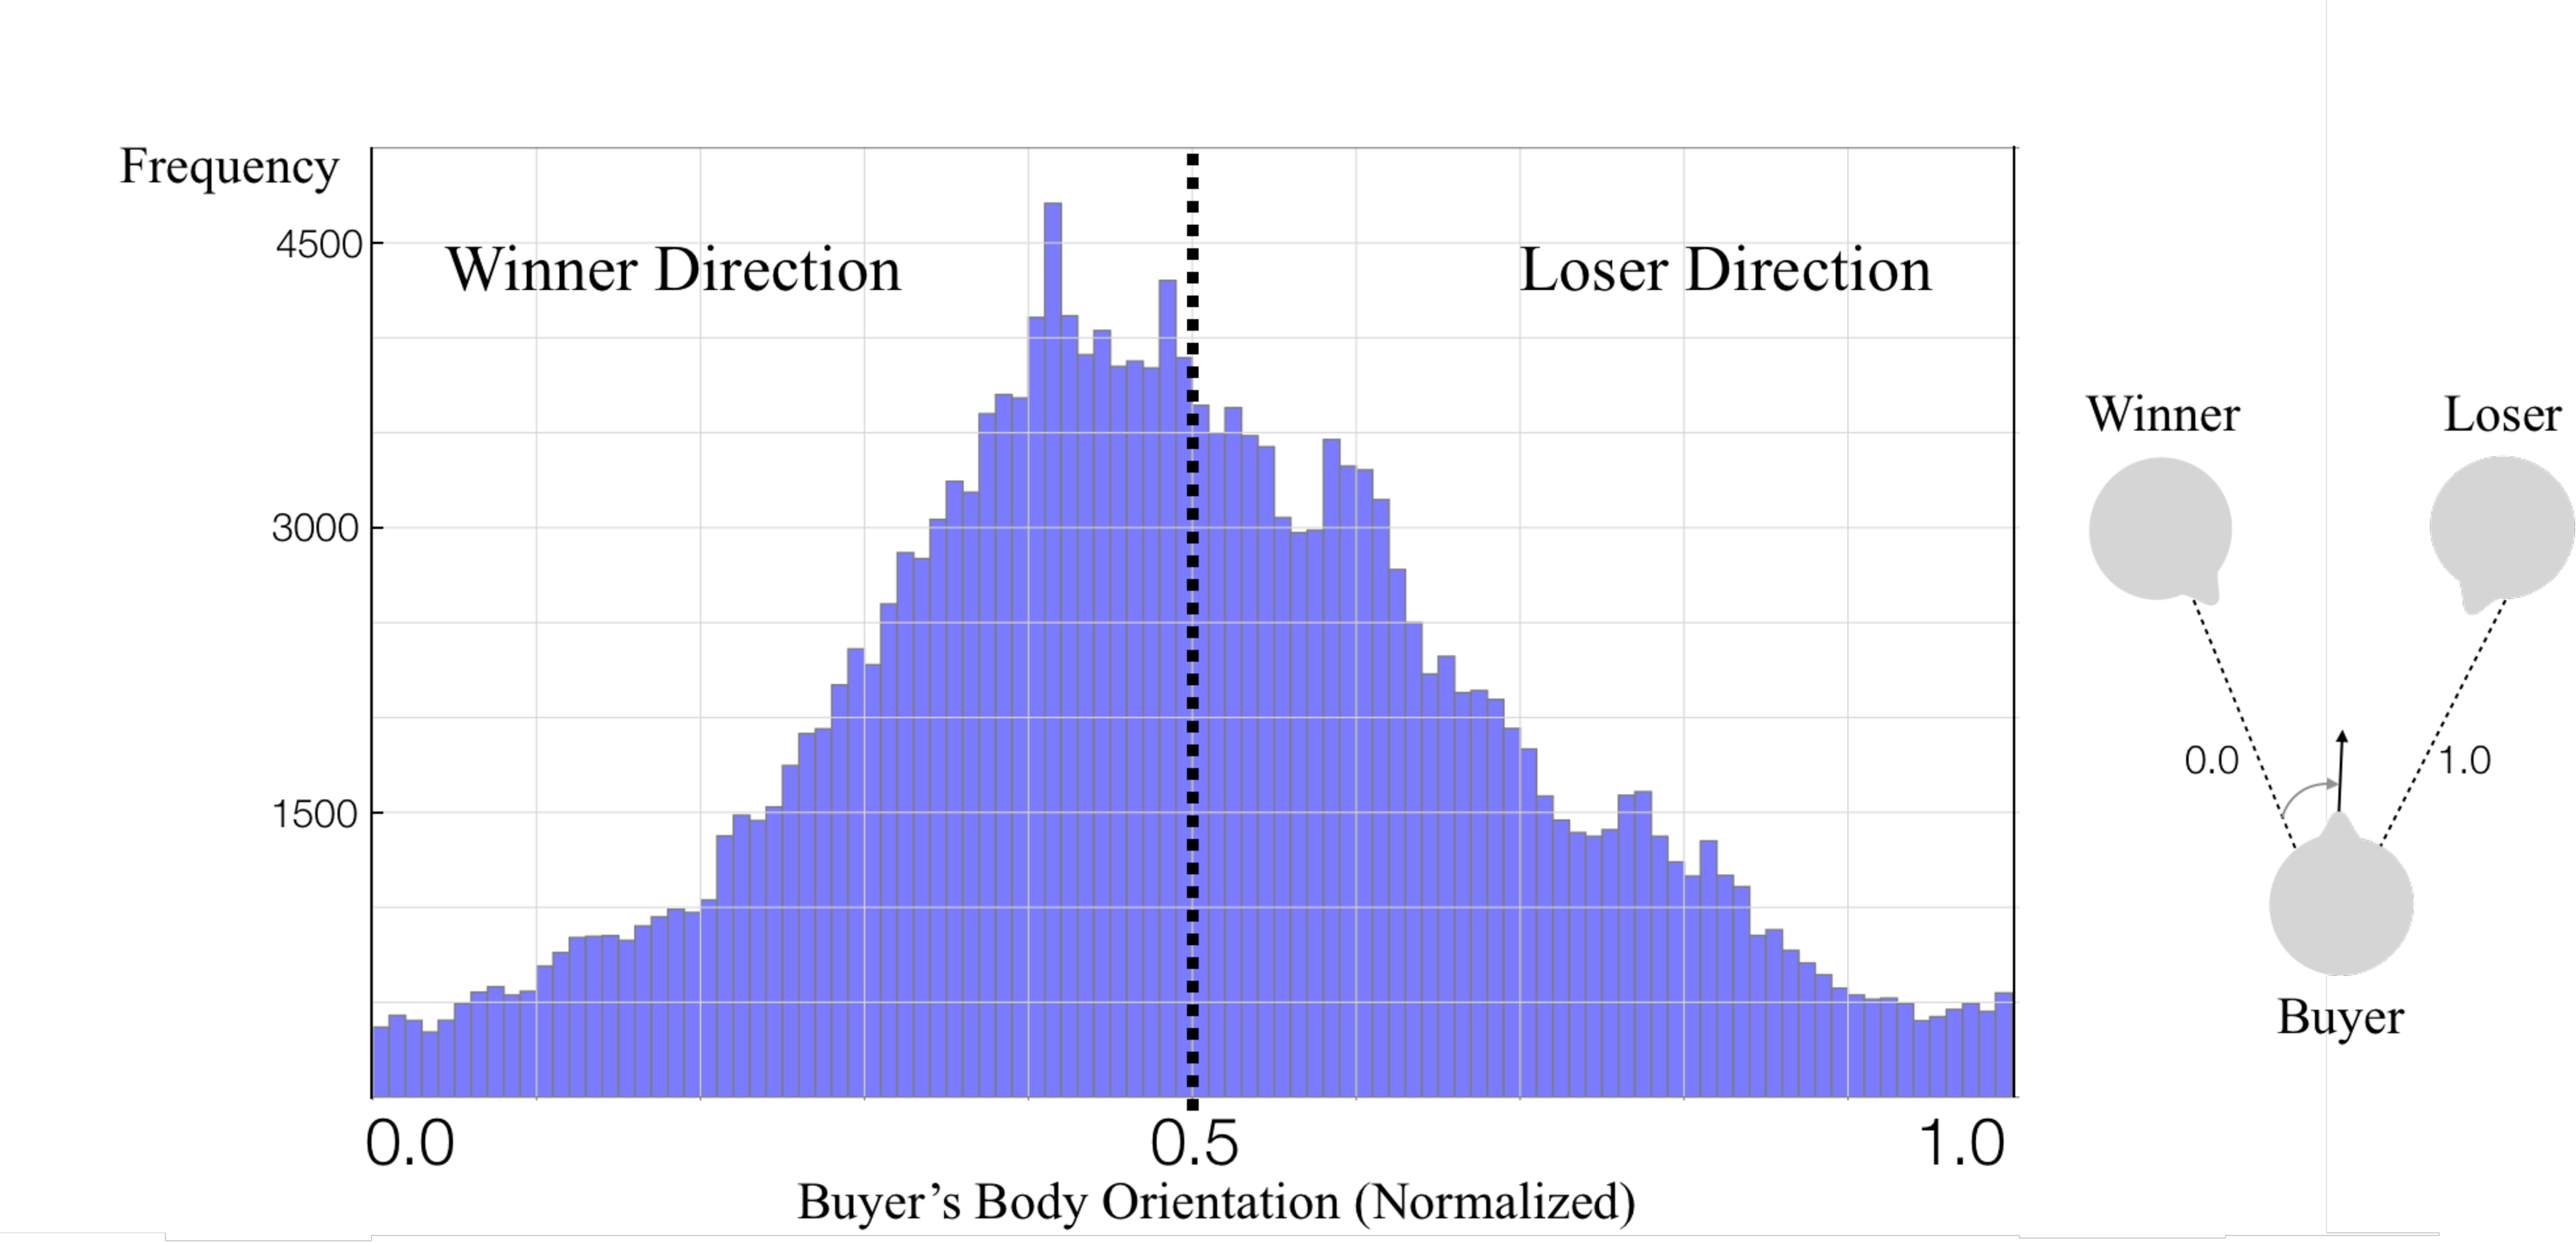
\includegraphics[width=\linewidth]{ssp_fig/result_buyer_bias}
	\caption{We can quantitatively verify whether there exists any bias in the body orientations of buyers toward winners. A histogram of the buyers' body orientation in a normalized orientation space is shown on the left by using entire haggling sequences. In this normalized orientation space, $0.0$ means that the buyer's body is fully facing the winner, and $1.0$ means that buyer's body orientation is fully facing the loser (as shown on the right figure).} 
	\label{fig:result_buyer_bias}
\end{figure}

\clearpage




% \subsection{Correlation between Body, Face, and Hands}

% We use all body parts for communication where each part plays a role to send some specific signals. Unfortunately, these roles are also poorly understood. In this section, we investigate whether there exists patterns or strong correlations among parts. We study this by predicting a missing part given other body parts. 

% Body2face, face2body

% \subsection{Face and Hands signals}